\chapter{Bibliographie}



\section{Qu'est ce qu'ANGULAR}
Angular est un framework Open Source développé par Google. Il est basé sur le langage JavaScript et est spécialisé sur la partie front-end\footnote{Partie du site web visible de l'utilisateur.}. Il utilise les possibilités offertes par HTML5 en créant des balises personnalisées.La vision de ce framework est de rendre le code HTML dynamique. On appelle cela un site en "Single Page Applcation"\footnote{Une application web monopage (en anglais single-page application ou SPA) est une application web accessible via une page web unique\cite{wiki:Single-page_application}}.

\section{L'historique du framework}

Ce framework a commencé son développement en 2009. La première version nommée AngularJS est quant à elle sortie en version 1.0.0 en 2012. Aujourd'hui, la  première version d'AngularJS est toujours maintenue et est disponible en version 1.6.3. Aujourd'hui Google propose une nouvelle version de son framework couramment nommée Angular 2. Cette version a été rendue disponible en version 2.0.0 en septembre 2016. La version actuellement en production est la version 2.2.0\cite{github:angular2}.

\begin{table}[h]
	\centering
	\begin{tabular}{|l|c|r|}
  		\hline
  			Date & Version & Note \\
  		\hline
		  2016-09-14 & 2.0.0 & Major Version Release \\
		  2016-10-12 & 2.1.0 & Minor Version Release \\
		  2016-11-09 & 2.2.0 & Minor Version Release \\
		  2016-12-14 & 4.0.0-beta.0 & \\
		  2017-03-22 & 4.0.0 + 2.4.12 & Major Version Release \\
  		\hline
\end{tabular}
	\caption{Release Schedule Angular}
\end{table}

Courant le mois de mars 2017, Google va diffuser une nouvelle version d'Angular couramment nommée Angular 4\label{angular4-release}. Elle devrait être disponible à partir du 22 mars 2017. Je détaillerais dans un prochain chapitre les nouvelles fonctionnalités apportées à cette version.
Google prévoit la sortie d'une nouvelle version majeure tous les 6 mois.

\section{ANGULAR 2, quoi de neuf ?}
Tout d'abord, ce qu’il faut savoir c'est que les versions AngularJS et Angular 2 (récemment renommé Angular tout court), n'ont pas grand-chose en commun. En effet l'équipe de développement a décidé de réécrire complètement le coeur de son framework et utilisant des technologies en devenir, nous allons revenir sur ce point.

Cette décision n'est pas sans conséquences. En effet le passage de la version 1.x a la version 2.0 implique une réécriture complète sans compatibilité ascendante du code et nous allons voir pourquoi.

\subsection{ECMAScript 6}

ECMAScript est l'appellation standardisée du JavaScript. Actuellement nous utilisons la version 5 dans nos développements JavaScript. Cepedant, on attend de plus en plus parler d'une nouvelle version du JavaScript nommé ECMAScript 6 ou ECMAScript 2015 ou encore ES6. En réalité, c'est la prochaine version majeure du langage JavaScript.

\paragraph{Mais pourquoi en parle-t-on ici ?}
Lors du passage à la version 2 d'Angular les développeurs ont voulu faire bénéficier de l'ES6 à leur framework pour le rendre plus moderne et l'ancrer dans l'avenir du développement web. Même s'il est toujours possible d'utiliser le JavaScript "standard", nous pouvons donc bénéficier des avantages de L4ES pour pour développer en Angular.

\paragraph{ES6, c'est quoi ?}
Comme décrit plus tôt ES6 est la prochaine version du JavaScript. Celle-ci a d'ailleurs atteint son état final récemment. Cependant, elle n'est pas encore supportée par tous les navigateurs. Pour pouvoir en bénéficier actuellement il faut utiliser un transpileur qui aura pour but de compiler l'ES6 dans sa version antécédente, c'est-à-dire l'ES5. Les deux outils actuellement les plus répandues sont Traceur\footnote{Projet développé par Google} et BabelJs\footnote{Projet développé à l'origine par Sebastian McKenzie (17 ans) et soutenu par une forte communauté et donc plus populaire}. Malheureusement certaine fonctionnalité de l'ES6 ne peuvent pas être transpileur en ES5.

\paragraph{Quoi de nouveau dans l'ES6?}
L'ES6 n'étant pas l'objet de ce rapport, je ne vais détailler que quelques évolutions qui me paraissent intéressantes.

\subsubsection{Déclaration de variable avec let}
En JavaScript, pour déclarer une variable on utilise le mot clé "\texttt{var}". Cette déclaration peut poser quelques problèmes. En effet en JavaScript, le concept de hosting\cite{ninja:angular} peut porter à confusion. Ce concept amène à déclarer la variable en tout début d'une fonction, peut l'endroit où elle a été codée. Voici un exemple pour illustrer:
\begin{lstlisting}[style=htmlcssjs, caption={Déclaration d'un bloc if}]
	function getUserFullName(user) {
  		if (user.isChampion) {
   			var name = 'Champion ' + user.name;
    			return name;
  		}
  		return user.name;
	}
\end{lstlisting}

\begin{lstlisting}[style=htmlcssjs, caption={Déclaration d'un bloc if equivalent}]
function getUserFullName(user) {
	var name;
  	if (user.isChampion) {
   		name = 'Champion ' + user.name;
    	return name;
  	}
  	return user.name;
}
\end{lstlisting}


Avec ES6, un nouveau mot clé est arrivé pour contourner ce problème, c'est \texttt{let}. Celui se comporte comme on peut l'attendre, voici un exemple : 

\begin{lstlisting}[style=htmlcssjs, caption={Déclaration d'un bloc if avec let}]
function getUserFullName(user) {
  	if (user.isChampion) {
   		let name = 'Champion ' + user.name;
    		return name;
  	}
  	// la variable name n'est pas accessible ici
  	return user.name;
}
\end{lstlisting}
Dans le même esprit, l'ES6 apporte la possibilité de créer des constantes avec le mot clé \texttt{const}. Comme pour les variables déclarées avec \texttt{let}, les constantes ne sont pas hoisted\footnote{"remontées"} et sont bien déclarée dans leur bloc.
\subsubsection{Les classes}
Une des nouvelles fonctionnalités importantes apportées par l'ES6 est l'arrivée de l'utilisation des classes en JavaScript.\label{ts-classes}. On pourra ainsi faire plus aisément de l'héritage de classes. Voici un exemple : 

\begin{lstlisting}[style=htmlcssjs, caption={Une classe avec héritage en ES6}]
class Vehicule {
  speed() {
    return 10;
  }
}

class Car extends Vehicule {
  speed() {
    return super.speed() + 10;
  }
}

const car = new Car();
console.log(car.speed()); // return 20.
\end{lstlisting}

\subsubsection{Arrow Functions}
Une des nouveautés de l'ES appréciée par les développeurs est la nouvelle syntaxe arrow functions\footnote{"fonction fléchée"} qui est utilisé principalement pour les callbacks et les fonctions anonymes. Cette syntaxe utilise l'opérateur => pour déclarer la fonction. La particularité des arrow functions est que le \texttt{this} reste attaché lexicalement, ce qui signifie que ces arrow functions n’ont pas un nouveau \texttt{this} comme les fonctions normales.Voici un exemple de son utilisation :
\begin{lstlisting}[style=htmlcssjs, caption={Exemple d'Arrow Function}]
const maxFinder = {
  max: 0,
  find: function (numbers) {
    numbers.forEach(element => {
      if (element > this.max) {
        this.max = element;
      }
    });
  }
};

maxFinder.find([2, 3, 4]);
// log the result
console.log(maxFinder.max);
\end{lstlisting}


Voici donc quelques notions importantes pour la suite de ce rapport sur l'utilisation d'Angular 2, mais très minimes quant à la quantité de nouveauté apportée par l'ES6. 

\subsection{TypeScript}

Le TypeScript est un langage développé par Microsoft dans le but de sécuriser la programmation JavaScript\cite{wiki:TypeScript}. C'est un langage libre et open source qui est un surensemble du JavaScript. Le TypeScript n'est donc pas un langage compris par les navigateurs et nous avons donc besoin d'utiliser un transpileur pour l'utiliser.
\begin{figure}[h]
	\centering
	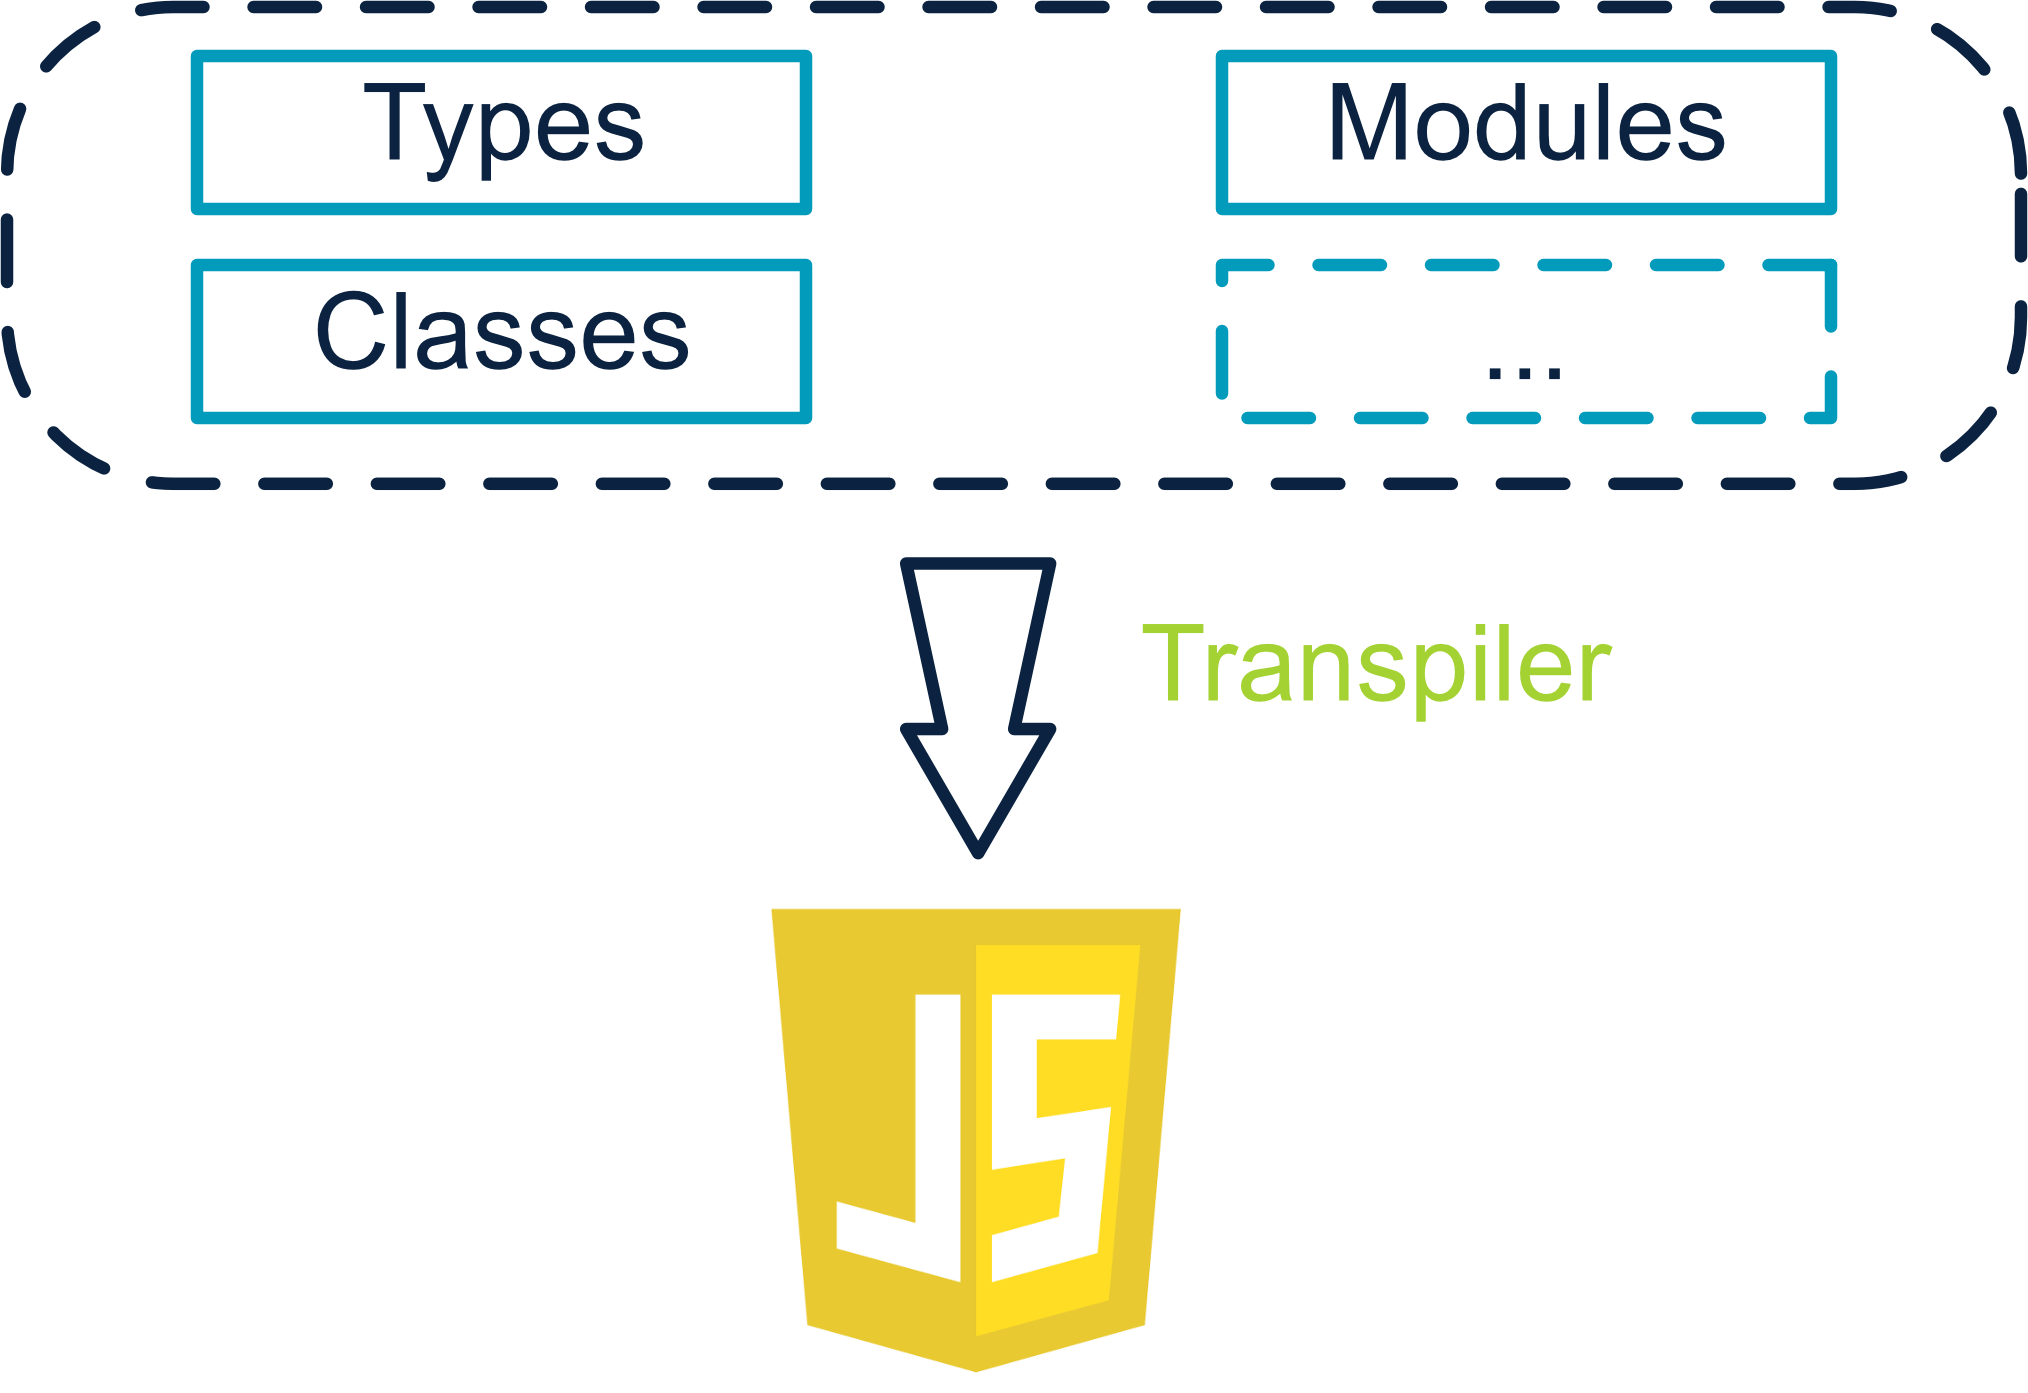
\includegraphics[scale=0.7]{typescript}
	\caption{Le TypeScript}
\end{figure}
Le transpileur, comme pour l'ES6, a pour but de rendre le code compréhensible par les navigateurs actuels. Il le convertit donc en ES3 ou ES5.

\paragraph{Un surensemble de quoi ?}
Le TypeScript a pour but d'améliorer la qualité et la sécurité du code JavaScript. Pour cela, il ajoute de nouvelles notions manquantes au JavaScript. 

\subsubsection{Le typage}
Comme le nom du langage le laisse suggérer, Le TypeScript apporte le typage au JavaScript\cite{grafikart:TypeScript}. Ainsi nous allons pouvoir définir un type à nos variables et/ou nos fonctions. Ce type peut être implicite ou explicite. Voici des exemples :

\begin{lstlisting}[style=htmlcssjs, caption={Typage explicite}]
let a: number

function demo(selector: string, options: {ease: string, duration: number}): Element{
    return document.querySelector(selector)
}
\end{lstlisting}

\begin{lstlisting}[style=htmlcssjs, caption={Typage implicite}, label={ts-typage-explicite}]
let a = 3
a = "Salut les gens" // Type 'string' is not assignable to type 'number'
\end{lstlisting}
Comme on peut le voir dans l'extrait de code \ref{ts-typage-explicite}, ce code n'est pas correct. C'est dans ce type de cas que l'on aborde la notion de sécurité du code. En effet ici, le transpileur donnera une erreur, car il s'attend à avoir un type \texttt{number}, défini ici implicitement à la première ligne. Mais à la deuxième ligne, on essaye d'affecter la valeur \texttt{"Salut les gens"} qui est de type \texttt{string}.



\subsubsection{Les classes}
Pourquoi reparle-t-on des classesdans le TypeScript alors que nous les avons déjà abordés en ES6 ? En effet nous avions vu dans le chapitre \ref{ts-classes} que l'ECMAScript 6 apportait la gestion des classes par le mot clé \texttt{class}. Cependant le TypeScript va encore plus loin. En effet, le langage permet de gérer la visibilité des différentes propriétés et la gestion des méthodes statiques comme en JAVA ou encore en PHP. Voici un exemple de code \cite{grafikart:TypeScript}

\begin{lstlisting}[style=htmlcssjs, caption={Les classes en TypeScript}]
class Demo {
    private factor

    constructor (factor: number) {
        this.factor = factor
    }

    public multiplie (n: number): number {
        return n * this.factor
    }

    static salut (): string {
        return 'Salut'
    }
}
\end{lstlisting}
Tout comme dans les langages orientés objet, il est possible de définir des accesseurs et des mutateurs avec les mots clé \texttt{set} et \texttt{get}.

\subsubsection{Les interfaces}
Avec TypeScript, il y a deux manières d'utiliser les interfaces. Il y a ma méthode "standard" connue dans d'autres langages de programmation qui consiste à implémenté une interface à une classe pour quelle en définissent les méthodes établies dans l'interface. La deuxième méthode d'implémentation dans le TypeScript est plus tournée vers l'utilisation des objets en JavaScript. En effet, l'on peut à l'aide de cette méthode définir la structure d'un objet que l'on attend en paramètre d'une fonction par exemple. Voici quelques lignes de code pour mieux comprendre :
\begin{lstlisting}[style=htmlcssjs, caption={Les interfaces en TypeScript}]
interface User {
    username: string;
    password: string;
    confirmPassword?: string; // Propriete optionnelle
}

let user:User;

user = {username: 'max', password: 'supersecret'};

// Les interfaces peuvent aussi contenir des fonctions

interface CanDrive {
    accelerate(speed:number): void;
}

let car:CanDrive = {
    accelerate: function (speed:number) {
        // ...
    }
};
\end{lstlisting}

\subsubsection{Les décorateurs}
Les décorateurs ne sont apparus qu'à partir de la version 1.5 de TypeScript et spécialement pour supporter Angular\cite{ninja:angular}. Le décorateur est une façon de faire de la métaprogrammation, ressemblant aux annotations qui sont utilisées en Java par exemple. La puissance des décorateurs réside dans le fait qu'ils peuvent modifier les paramètres ou encore le résultat retourné. Ils peuvent également appeler d'autres méthodes quand la cible est appelée ou ajoutée de métadonnées, c'est ce qui est notamment utilisé pour l'utilisation avec le framework Angular. Dans TypeScript les décorateurs sont préfixés d'un \texttt{@}.

Le bémol de cette solution c'est qu'elle est encore au stade expérimental\cite{ts:decorator}. Cependant il y a de bonnes chances que cela soit supporté officiellement à l'avenir (peut-être dans ES7 ?).

\begin{lstlisting}[style=htmlcssjs, caption={Exemple de décorateur dans Angular}]
@Component({ selector: 'ns-home' })
class HomeComponent {

  constructor(@Optional() hello: HelloService) {
    logger.log(hello);
  }

} 
\end{lstlisting}
Dans cet exemple le décorateur est \texttt{@Component}. Il est ajouté à la classe \texttt{Home}. Cela permet a Angular de comprendre au chargement que cette classe est un composant.

\paragraph{Pourquoi utiliser le TypeScript ?}
La question que l'on peut se poser quand on découvre le TypeScript est de savoir quel est l'intérêt par rapport au JavaScript, puisque le code TypeScript est transpileur en JavaScript. Tout d'abord, il y a des raisons assez générales et des raisons plus spécifiques a l'utilisation d'Angular. Une première raison est que ce langage est beaucoup moins libertaire que le JavaScript, dans le but d'avoir un code plus sécurité. Le typage permet de vérifier la cohérence des déclarations et des utilisations de variables et de fonction. De plus, la plupart des IDE tirent un avantage important de ce typage pour mettre en avant les erreurs de code ou permettre l'autocompletion. Ensuite le TypeScript utilise l'avantage de l'ES6 et pali au manque du JavaScript actuel en utilisant les classes, les interfaces et encore bien d'autres nouveautés.

Angular se base principalement sur le TypeScript. Si l'on regarde la documentation d'Angular\cite{angular:doc}, on peut voir qu'il existe une version d'Angular pour JavaScript ou encore pour Dart. Cependant actuellement la version la mieux documentée et la plus soutenue par la communauté et Google est la version écrite en TypeScript.

Il est donc largement préférable d'utiliser le langage TypeScript si vous voulez faire de l'Angular.

\subsection{Web Component}
La notion de composant dans le monde du web n'est pas nouvelle, elle était déjà apparue dans d'autres frameworks comme jQuery ou encore dans la première version d'Angular (AngularJS). Ces composants avaient le défaut de nécessité de nombreuse dépendance ce qui rendait le code complexe. Avec Angular 2, Google a voulu corriger le problème en proposant d'avoir des Web Components\footnote{composants web} réutilisables et encapsulés, c'est à dire avec leur propre logique, leur propre affichage. Il repose sur quatre spécifications\cite{ninja:angular} :

\begin{itemize}
	\item Custom Elements\footnote{éléments personnalisés}, sont des éléments du DOM créé par le développeur en fonction de ses besoins. Il peut alors créer des balises HTML personnalisées par exemple \texttt{<ng-app></ng-app>}.
	\item Shadow DOM\footnote{DOM de l'ombre} est un moyen d'encapsuler le DOM d'un composant dans le DOM principal. Cela permet de séparer le style et la logique de programmation de l'application globale de celle du composant.
	\item Le template, spécifié dans un élément \texttt{<template>} n’est pas affiché par le navigateur. Son but est d’être à terme cloné dans un autre élément. Ce qui est déclaré à l’intérieur sera inerte : les scripts ne s’exécuteront pas, les images ne se chargeront pas, etc. Son contenu peut être appelé par le reste de la page avec la méthode classique \texttt{getElementById()} et il peut être placé sans risque n’importe où dans la page.
	\item HTML Imports, ils permettent d'importer du HTML dans du HTML. Cela permet un code réutilisable facilement.
\end{itemize}
Il faut noter que ces standards ne sont pas encore tout à fait supportés par les navigateurs, Chrome étant le plus avancé sur ce point.

\subsection{ANGULAR CLI}
Un autre apport de la version 2 d'Angular et l'arrivée d'un outil de gestion de l'application Angular par ligne de commandes. Cet outil, nommé Angular CLI\footnote{Angular Command Line Interface}, permets de gérer facilement le développement de l'application. Un prérequis est nécessaire pour son utilisation, il faut avoir installé localement NodeJS ainsi que le gestionnaire de paquet NPM \cite{angluar:cli}.
\paragraph{ng new}
Le CLI permet tout d'abord la création de l'application en elle même en créant la structure et le fichier standards et nécessaire pour que le framework fonction.
\begin{lstlisting}[language=bash]
ng new my-project
\end{lstlisting}
Cette commande va donc générer les fichiers dans un dossier nommé \texttt{my-project}.

\paragraph{ng serve}
Une autre commande importante du CLi est la commande \texttt{ng serve}. Celle-ci permet le lancement d'un serveur qui s'exécute en arrière-plan pour compiler l'application et la rendre utilisable en développement. De plus, toutes les modifications seront mises à jour en direct sur le navigateur ce qui est un vrai confort de programmation. L'application est accessible à l'adresse \texttt{http://localhost:4200/}

\paragraph{ng generate}
La commande ng generate est sûrement la plus utilisée dans le développement Angular. En effet cette commande est centrale, elle permet de générer les principaux éléments sur lesquels nous allons travailler.
\begin{lstlisting}[language=bash]
ng generate class // generer une class
ng generate component // generer un composant
ng generate interface // generer une interface
// ...
\end{lstlisting}
Cette commande va non seulement générer les différents fichiers, mais va aussi les déclarer dans le fichier de gestion de modules pour les rendre utilisables. Ce point sera détaillé dans la deuxième partie du rapport. C'est donc un vrai confort d'utilisation qui évite d'éditer une multitude de fichiers avant de pouvoir réellement coder le nouvel élément généré
\paragraph{ng build}
La dernière commande que je vais aborder, il y en a plusieurs d'autres\cite{angluarcli:doc}, c'est \texttt{ng build}. Cette commande, comme on peut s'en douter permet de créer l'application finale pour la mise en production. En effet, avec cette commande est créé un dossier dans \texttt{dist} dans le projet qui contient l'application compilée en JavaScript et qui pourra être hébergée sur un serveur.

\section{Angular 4, prochaine version majeure}
Comme je l'ai abordé au chapitre \ref{angular4-release}, une nouvelle version d'Angular devrait sortir dans les prochains jours (mars 2017). Cette version sera donc Angular 4. 
\paragraph{Mais où est passé Angular 3 ?}
Il se trouve qu'actuellement nous utilisons déjà une partie d'Angular 3 sans même le savoir. En effet, le module de routage actuellement utilisé est en version 3.2.3. Pour une question de clarté et d'harmonisation, l'équipe de développement d'Angular a donc décidé de passer directement à la version 4 pour limiter les confusions.

\paragraph{Qu'apporte de nouveau Angular 4 ?}
Tout d'abord, l'équipe de développement a tenu à rassurer les développeurs utilisant leur framework, passer de la version 2 a la version 4 demandera bien moins d'effort que lorsque nous étions passés de la version "1" a la version 2\cite{youtube:angular4annoncement}.
Voici les nouveautés attendues de cette version :
\begin{itemize}
	\item TypeScript 2.1 pour tirer les avantages de cette nouvelle version.
	\item Rétro compatibilité avec Angular 2
	\item Meilleur compileur Angular
	\item Gain de rapidité
	\item Réduction de la taille 
\end{itemize}

\section{D'autres frameworks}
Il existe d'autres frameworks front-end sur le marché qui prennent le parti du Web Component. En effet, Facebook a notamment développé sa propre solution et l'utilise pour son site phare, il s'agit de ReactJS. EmberJS lui se rapproche de la façon dont fonctionnait AngularJS. Enfin, il existe des frameworks plus récents, tels que VueJS ou encore le petit dernier Aurelia, qui sont plus spécialisés dans la création de petits composants web sans fournir les services autour, comme le fait Angular. Il faut alors passer par des librairies tierces pour ajouter les fonctions que l'on souhaite.
\begin{figure}[h]
	\centering
	
\includegraphics[scale=1.2]{Autres_frameworks}
	\caption{EmberJS, Aurelia, ReactJS, VueJS}
\end{figure}
